% !TEX root = ../BScWIMEngl.tex  

\chapter{Markov Decision Processes}
\section{Introduction}
In this introduction I try to convey an intuition for Markov Decision Processes. Readers familiar with the subject can skip directly to the more formal model formulation. 

A Markov Decision Process appears to be quite similar to a Markov Process at first glance. Where a Markov Process is a stochastic process, i.e. a sequence of random variables \((X_t,t\in\N_0)\), which is memoryless (Markov). That means knowledge of the current state, makes knowledge about past states useless for predicting future states.

Markov Decision Processes (MDPs) introduce actions \((A_t,t\in\N_0)\) and rewards \((R_t,t\in\N)\) to this model. Where the transition to the next state \(X_{t+1}\) given a state \(X_{t}\) and action \(A_{t}\) is markov (memoryless) just like in case of Markov Processes.
\[
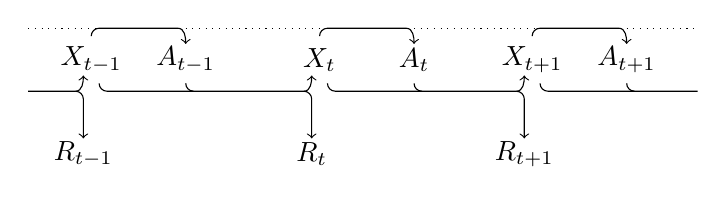
\begin{tikzpicture}
    \draw[dotted] (-3.7,0.4) -- (-2.8,0.4);

    \draw[->] (-3.7, -0.4) %%% transition stub beginning
    to [out=0,in=180] (-3.1, -0.4)
    to [out=0,in=270] (-3, -0.2);

    \draw[->] (-3.1, -0.4) %%% to R_{t-1}
    to [out=0,in=90] (-3,-0.5)
    to [out=270, in=90] (-3,-1);

    \draw (-3,-1.2) node {\(R_{t-1}\)};
    \draw (-2.9,0) node {\(X_{t-1}\)};

    \draw[->] (-2.9,0.3) %%% X_{t-1} to A_{t-1}
    to [out=90,in=180] (-2.8, 0.4) 
    to [out=0,in=180] (-1.8,0.4)
    to [out=0,in=90] (-1.7,0.2);

    \draw[dotted] (-1.7,0.4) -- (0.1,0.4);

    \draw (-1.7,0) node {\(A_{t-1}\)};

    \draw (-1.7, -0.3) %%% join transition 
    to [out=270,in=180] (-1.6,-0.4);

    \draw[->] (-2.8, -0.3) %%% X_{t-1} to X_t transition
    to [out=270,in=180] (-2.7, -0.4) 
    to [out=0,in=180] (-0.2, -0.4)
    to [out=0,in=270] (-0.1, -0.2);

    \draw[->] (-0.2, -0.4) %%% to R_t
    to [out=0,in=90] (-0.1,-0.5)
    to [out=270, in=90] (-0.1,-1);

    \draw (-0.1,-1.2) node {\(R_t\)};
    \draw (0,0) node {\(X_t\)};
    
    \draw[->] (0,0.3)  %%% X_t to A_t
    to [out=90,in=180] (0.1, 0.4) 
    to [out=0,in=180] (1.1,0.4)
    to [out=0,in=90] (1.2,0.2); 

    \draw[dotted] (1.2,0.4) -- (2.8,0.4);
 
    \draw (1.2,0) node {\(A_t\)};

    \draw (1.2, -0.3) %%% join transition
    to [out=270,in=180] (1.3,-0.4);

    \draw[->] (0.1, -0.3) %%% X_t to X_{t+1} transition
    to [out=270,in=180] (0.2, -0.4) 
    to [out=0,in=180] (2.5, -0.4)
    to [out=0,in=270] (2.6, -0.2);

    \draw[->] (2.5, -0.4) %%% to R_{t+1}
    to [out=0,in=90] (2.6,-0.5)
    to [out=270, in=90] (2.6,-1);

    \draw (2.6,-1.2) node {\(R_{t+1}\)};
    \draw (2.7,0) node {\(X_{t+1}\)};

    \draw[->] (2.7,0.3)  %%% X_{t+1} to A_{t+1}
    to [out=90,in=180] (2.8, 0.4) 
    to [out=0,in=180] (3.8,0.4)
    to [out=0,in=90] (3.9,0.2); 

    \draw[dotted] (3.9,0.4) -- (4.8,0.4);

    \draw (3.9,0) node {\(A_{t+1}\)};

    \draw (3.9, -0.3) %%% join transition stub
    to [out=270,in=180] (4,-0.4);

    \draw (2.8, -0.3) %%% X_{t+1} transition stub end
    to [out=270,in=180] (2.9, -0.4) 
    to [out=0,in=180] (4.8, -0.4);
\end{tikzpicture}
\]
But this apparent similarity can be misleading. While Markov Processes are defined as a stochastic process (i.e. a sequence of states) with properties as described above, MDPs cannot be defined like that. The reason for this is, that the next state \(X_{t+1}\) depends on the current state and action \(A_{t}\), which means that the sequence of states cannot be defined without the sequence of actions. But defining the sequence of actions requires an action selection rule, a behavior, a decision. So defining MDPs as a stochastic process, would result in every behavior resulting in a different MDP. But since MDPs want to model decisions, this does not make much sense. Talking about optimal behaviors in a framework which can only be defined for a set behavior, is nonsensical. What is needed is a model framework which is invariant to different behaviors. Therefore MDPs are not defined as a stochastic process, but rather as a rulebook on how to create a stochastic process from a given behavior. 

The questions we ask the model are also different.  MDPs are more interested into evaluating different behaviors and finding optimal ones, while Markov Processes try to describe an existing phenomenon. Though we will find, that -- given a behavior which is memoryless as well (without the dotted lines in the diagram) -- the resulting stochastic process \((X_t,A_t,R_{t+1},t\in\N_0)\) is a Markov Process, so the theory of Markov Processes could in principle be applied. But this will not be our focus. 

Just like with Markov Chains, the memorylessness could be circumvented by including the history in the current state, massively increasing the state space in the process. Which means it is questionable whether this would yield any interesting results, as then no state is visited twice. So it is of no use to an actor to learn the value of an action in a certain state without further assumptions.

To illustrate the uses of such a framework, I have selected a few examples from \textcite{whiteRealApplicationsMarkov1985}:
\begin{enumerate}
	\item Resource Management: The state is the resource level
	\begin{itemize}
		\item Inventory Management: The resource is the inventory, the possible action is to order resupply, influencing the inventory (state) together with the stochastic demand, and the reward is the profit. The essential trade-off is the cost of storage versus lost sales from a stock-out.
		\item Fishing: The resource is the amount of fish, the action is the amount fished, the reward is directly proportional to the amount fished, and the repopulation is the random element.
		\item Pumped storage Hydro-power: The state is the amount of water in the higher reservoir and the electricity price, the action is to use water to generate electricity or wait for higher prices.
		\item Beds in a hospital: How many empty beds are needed for emergencies?
	\end{itemize}
	\item Stock trading: The state is the price level and stock and liquidity owned.
	\item Maintenance: When does a car/road become too expensive to repair?
	\item Evacuation in response to flood forecasts
\end{enumerate}
Lastly, to ease ourselves into the abstract definition of MDPs, let us do one example in more depth.
\begin{example}[Inventory Management]\label{example: inventory mgmt} We will look at a retail store with just one good for simplicity. Let
	\begin{description}[noitemsep]
		\item[\(\cX\coloneqq\N\)] be the set of possible quantities of goods in stock,
		\item[\(\cA\coloneqq\N\)] be the set of possible orders for resupply.
	\end{description}
	We will now introduce the mechanics of actions and rewards without stochastic behavior and then change that later.

	Let us assume that the ordered goods \(a_t\in\cA\) arrive in the morning the next day. The goods sold are the demand \(d_t\), if the current stock \(x_t\in\cX\) can meet the demand. So the amount sold is actually \(d_t\wedge x_t = \min\{d,x_t\}\). Assume orders are paid for in advance and bought at price \(1\), while the goods are sold at price \(p\). The cost of storage is \(q\) per item and day. Then the profit at the end of day \(t\) is
	\[
		r_{t+1}= p (d\wedge x_t)-a_t-q(x_t - d\wedge x_t)
	\]
	And the stock level on the next day will be
	\[
		x_{t+1}=x_t - d_t\wedge x_t + a_t 
	\]
	We express this with the \emph{state transition function} \(f\) defined as
	\begin{align*}
		&f(x,a,d)\coloneqq \left(x-d\wedge x + a,\; p(d\wedge x) - a - q(x - d\wedge x)\right)\\
		&\implies f(x_t,a_t,d_t)=(x_{t+1}, r_{t+1})
	\end{align*}
	Now assume that the demand is a random variable \(D_t\) which are independent and identically distributed (iid) for all \(t\). This makes all the other objects (except for the actions) neccessarily random variables too. Then distribution of \((X_{t+1},R_{t+1})\) conditional on \(X_t=x, A_t=a\) is defined to be the \emph{transition probability kernel} \(\cP\) with
	\begin{align*}
		\cP(\cdot \mid x, a)\coloneqq\Pr_{f(x,a,D_t)}\xeq{\text{iid}} \Pr_{f(x,a,D_0)}
	\end{align*}
	Note that knowledge of the transition kernel \(\cP\) is equivalent to knowledge of the transition function \(f\) and the distribution of the demand. Transition kernels reduces the clutter caused by exogenous random variables which are different from application to application and are unknown until the next state is realized at which point their knowledge is useless. We will therefore define this MDP to be \(\cM=(\cX,\cA,\cP)\).

	A stationary behavior in this example would be a probability distribution over the possible orders, given the current state
	\begin{align*}
		\pi(\cdot \mid x) \text{ Probability distribution over }\cA
	\end{align*}
	Actions are then selected by picking a random variable from this distribution
	\[
		A_t \sim \pi(\cdot \mid X_t)
	\]
	Non-stationary behaviors are probability distributions over the action space which can depend on the entire history of states, actions and rewards. 
\end{example}

We will just make one more generalization in the actual definition of MDPs. We will allow the action space \(\cA\) to depend on the state \(x\in\cX\).

\section{Model Formulation}
%countable state space
Most of the definitions in this chapter are adaptations from \textcite{szepesvariAlgorithmsReinforcementLearning2010}.
But to properly define the transition probabilities given an action in a certain state, let us define a probability kernel first.

\begin{definition}[Kernel]
	Let \((Y,\sigma_Y), (X,\sigma_X)\) be measure spaces.
	\begin{align*}
		&\lambda\colon X\times\sigma_Y\to \R \text{ is called a \emph{(probability) kernel}}\\
		&\qquad \qquad :\iff 
		\begin{aligned}[t]
			&\lambda(\cdot,A)\colon x\mapsto \lambda(x,A) \text{ measurable}\\
			&\lambda(x,\cdot)\colon A\mapsto \lambda(x,A) \text{ a (probability) measure}
		\end{aligned}
	\end{align*}
	Since we will interpret probability kernels as distributions over \(Y\) given a  certain condition \(x\in X\), the notation \(\lambda(\cdot\mid x) \coloneqq \lambda(x,\cdot)\) helps this intuition. 
\end{definition}

\begin{definition}
	\(\cM=(\cX,\cA,\cP) \) is called a \emph{(finite) Markov Decision Process} (MDP), where
	\begin{description}[noitemsep]
		\item[\(\cX\)] is a countable (finite) set of states,
		\item[\(\cA=(\cA_x)_{x\in\cX}\)] with \(A_x\) the countable (finite) set of possible actions in state \(x\),
		\item[\(\cP\colon (\cX\times\cA) \times \sigma_{\cX\times\R} \to \R\)] is a probability kernel, with the notation 
		\begin{align}\label{notation: XxA}
			\cX\times\cA\coloneqq \{(x,a): x\in\cX, a\in\cA_x \} 
		\end{align}
		\item[\(\cX\times\R\)] represents the next state and the reward. So \(\cP(\cdot\mid x,a) \) represents the probability distribution over the next states and rewards given an action \(a\) in the state \(x\).
		\item[\(\cP\)] is called the \emph{transition probability kernel}, or in short transition kernel.  
	\end{description}
\end{definition}
\begin{remark}\label{split state/reward transition kernel }
	Most authors split the transition kernel into a state transition kernel and a reward kernel \parencite[e.g.][]{putermanMarkovDecisionProcesses2005}. But since it is easier to define a marginal distribution from a joint distribution than vice versa, and since this notation is more compact I will stick to the definition from \textcite{szepesvariAlgorithmsReinforcementLearning2010}. 
	
	We will spare ourselves the complications of changing transition kernels over time. Just like the memorylessness this could be circumvented by including time in the state. But if an algorithm is to learn which actions are optimal in which state, then both changing transition kernels over time and state spaces where you never visit any state twice (since the time is included) make it impossible to learn ``the rules of the game'' without assumptions on how the rules change over time. If such assumptions can be made it is usually easier to bake them into the state space. For example if you would like to introduce changing demand distributions over time in our inventory management example (\ref{example: inventory mgmt}), you could add the current expected demand to the state. Also adding the current market penetration, changes in the demand distribution can be modelled with a stationary transition kernel. 
\end{remark}

According to \textcite{putermanMarkovDecisionProcesses2005} some authors call this tuple a Markov Decision Problem instead of Markov Decision Process, presumably to reserve the term Markov Decision Process for the resulting sequence of states, actions and rewards \((X_t,A_t,R_{t+1},t\in\N_0)\), aligning the Definition with the definition of a Markov process. Although this does not appear to be common practice.

Nevertheless we still need to construct that stochastic process from the MDP when we have an action selection rule. 

\fxnote{Make this a definition of some sort?}
First, we need to select the random variable \(X_0\) of the initial state. The initial state is not included in the definition of an MDP because later objects will be defined conditional on the current state. They are thus invariant to different starting distributions, as long as \(\Pr(X_0=x)>0\) holds for all \(x\in\cX\) ensuring that conditioning on every state is possible.

Second, we need an action selection rule

\begin{definition} 
	An \(A_t\) selection-rule \(\pi=(\pi_t,t\in\N_0)\) is called (history dependent) \emph{behavior (policy)}, where
	\[ 
		\pi_t\colon
		\begin{cases}
			(\cX\times\cA\times\R)^t\times\cX\times\sigma_{\cA} \to \R \\
			(h,x,A)\mapsto \pi_t(A\mid h,x)
		\end{cases} \text{ is a probability kernel,}
	\]
	and \(A_t\sim \pi_t(\cdot\mid (X_0,A_0,R_1), \dots,(X_{t-1},A_{t-1},R_t),X_t))\).
	\footnote{ 
		note that \(\cX\times\sigma_\cA\coloneqq \{(x,A): x\in\cX, A\in\sigma_{\cA_x} \} \) is defined just like \(\cX\times\cA\) (c.f. (\ref{notation: XxA}))
	 } \\
	The following special cases can be viewed as policy subsets with some abuse of notation:
	\begin{enumerate}
		\item \emph{Markov policies} \(\pi=(\pi_t,t\in\N_0)\) are memoryless policies, i.e.
		\[
			\pi_t\colon
			\begin{cases}
				\cX\times\sigma_{\cA} \to \R \\
				(x,A)\mapsto \pi_t(A\mid x)
			\end{cases} 
			\text{ with } A_t\sim \pi_t(\cdot\mid X_t)
		\]
		\(A_t\) is selected such that it has the markov property (well defined c.f. \ref{well defined markov property}), i.e.
		\[\Pr[A_t=a\mid X_t]=\Pr[A_t=a\mid X_t, (X_{t-1},A_{t-1},R_t), \dots (X_0,A_0,R_1)] \]
		\item \emph{Stationary policies} are policies which do not change over time i.e. \(\pi_{t+1}=\pi_t\). Since \(\pi_0\) can only depend on the first state, they are naturally markov and can be defined as
		\[
			\pi\colon 
			\begin{cases}
				\cX\times\sigma_{\cA}\to\R\\
				(x,A)\mapsto \pi(A\mid x)
			\end{cases} 
			\text{ with } A_t\sim\pi(\cdot\mid X_t) 
		\]
		\item \emph{Determinisitic stationary policies} are specified by\footnote{
			\(\pi\colon\cX\to\cA_x\) is notation for \(\pi\colon\cX\to\bigcup_{x\in\cX} \cA_x : \pi(x)\in\cA_x \)
		}
		\[
			\pi\colon\cX\to\cA_x \quad\text{ with }A_t=\pi(X_t)
		\]
	\end{enumerate}
	Similarly, deterministic markov policies and deterministic history dependent policies can be defined. The sets of these policies will be denoted like this
	\[
	\begin{tikzcd}[row sep = small, column sep = small]
		&\text{Stationary} & \text{Markov} & \text{History dependent}
		\\
		\text{Deterministic} 
		& \detPolicy
			\arrow[draw=none, shift right=2]{r}{\subseteq} 
			\ar[draw=none, shift right=2.7]{d}{\vsubseteq}
		& \Pi_M^D
			\arrow[draw=none, shift right=2]{r}{\subseteq} 
			\ar[draw=none, shift right=2.7]{d}{\vsubseteq}
		& \Pi^D
			\ar[draw=none, shift right=2.7]{d}{\vsubseteq}
		\\ 
		\text{Stochastic} 
		& \statPolicy 
			\arrow[draw=none, shift right=2]{r}{\subseteq} 
		& \Pi_M
			\arrow[draw=none, shift right=2]{r}{\subseteq}
		& \Pi
	\end{tikzcd}
	\]
\end{definition}

Now we define inductively: \((X_{t+1}, R_{t+1})\sim\cP(\cdot\mid X_t, A_t)\) with the Markov property (well defined c.f. \ref{well defined markov property}), i.e.
\begin{align}
\label{X,R Markov}
	&\Pr[(X_{t+1}, R_{t+1})=(x,r)\mid (X_t,A_t)]\\
	&=\Pr[(X_{t+1},R_{t+1})=(x,r) \mid (X_t,A_t),(X_{t-1},A_{t-1},R_t), 
	\dots (X_0,A_0,R_1)] \nonumber
\end{align}
resulting in the stochastic process \(((X_t,A_t,R_{t+1}), t\in \N_0)\)
\begin{remark}\label{well defined markov property}\fxnote{remark? lemma? prop?}
	\((X_{t+1}, R_{t+1})\sim\cP(\cdot\mid X_t, A_t)\) with the Markov property, is well defined i.e.:
	There exists a \(\cX\times\R\)-valued random variable \((X_{t+1}, R_{t+1})\)
	such that
	\begin{align*}
		(X_{t+1}, R_{t+1})\sim\cP(\cdot\mid X_t, A_t) \text{ and it satisfies the Markov property}
	\end{align*}
	(analogous \(A_t\) well defined)
\end{remark}
\begin{proof}
	As we want to use cumulative distribution functions (cdf) for this proof, we first embed the \(cX\times\R\) in \(\R\). Since \(\cX\) is countable there exists an injective measurable mapping \(g\colon \cX\to\N\)
	and because there exist an injective sigmoid function \(\sigma\colon \R\to(0,1)\), there exists an injective measurable function
	\begin{align*}
		f\colon
		\begin{cases}
			\cX\times\R \to \R \\
			(x,r)\to g(x)+\sigma(r)
		\end{cases}
	\end{align*}
	This allows us to define a probability kernel on the real numbers and the corresponding cdf
	\begin{align*}
		\tilde{\cP}(\cdot\mid x,a)&\coloneqq \Pr_{f\circ Y} \text{ where } Y\sim \cP(\cdot\mid x,a)\\
		F_{x,a}(y)&\coloneqq \tilde{\cP}( (-\infty,y]\mid x,a)
	\end{align*}
	Now we select \(U\sim \cU(0,1)\) independent from the entire history, then 
	\begin{align*}
		F^\leftarrow_{x,a}(U) \sim \tilde{\cP}(\cdot\mid x,a) 
		\ximplies{\text{\ref{appx2}}} f^{-1}\circ F^\leftarrow_{x,a}(U)\sim \cP(\cdot \mid x,a)
	\end{align*}
	where \(F^\leftarrow\) is the pseudo-inverse (\ref{appx3}).	Thus 
	\[
		(X_{t+1},R_{t+1})\coloneqq f^{-1}\circ 
		F^\leftarrow_{X_t, A_t}(U) \sim \cP(\cdot \mid X_t, A_t)
	\]
	fulfills the first requirement and is also markov. To show the markov property we first define a shorthand for the history
	\[
		\cH_s^t\coloneqq \{(X_t,A_t,R_{t+1})\in H_t,\dots,(X_s,A_s,R_{s+1})\in H_s \}
	\]
	where \(H_i\) is defined as
	\[
		H_i\coloneqq\{(x_i,a_i)\}\times U_i \in \sigma_{\cX\times\cA\times\R}
	\]
	With this notation we can now finish the proof
	\begin{align*}
		\Pr(f^{-1}\circ F^\leftarrow_{X_t, A_t}(U) \in A \mid \cH_0^t)
		&=\frac{\Pr(f^{-1}\circ F^\leftarrow_{x_t, a_t}(U) \in A, \cH_0^t)}{
			\Pr(\cH_0^t)}\\
		&\lxeq{\text{U indep.}}\Pr(f^{-1}\circ F^\leftarrow_{x_t, a_t}(U) \in A)\\
		&=\dotsc = \Pr(f^{-1}\circ F^\leftarrow_{X_t, A_t}(U) \in A \mid \cH_t^t)\qedhere
	\end{align*}
\end{proof}

\begin{prop}\label{statPolicy induces time-homogeneous MC}
	A (stationary) markov  policy \(\pi\) induces a (time homogeneous) Markov chain \((X_t,A_t,R_{t+1},t\in\N_0)\).
\end{prop}
\begin{proof} 

	Using the shorthand for the history defined in the last proof together with 
	\[
		\Pr(A\cap B \mid C)
		=\frac{\Pr(A\cap B\cap C)}{\Pr(B\cap C)}\frac{\Pr(B\cap C)}{\Pr(C)} 
		= \Pr(A\mid B\cap C)\Pr(B\mid C) 
	\]
	we can show the Markov property of the resulting chain
	\begin{align}
		&\Pr\left[(X_t,A_t,R_{t+1})\in\{(x,a)\}\times U \mid \cH_0^{t-1} \right] \nonumber \\
		&=\Pr\left[R_{t+1}\in U \mid (X_t, A_t)=(x,a), \cH_0^{t-1}\right]
		\Pr\left[(X_t, A_t)=(x,a)\mid\cH_0^{t-1}\right]
		\nonumber\\
		&\lxeq{(\ref{X,R Markov})}\Pr\left[R_{t+1}\in U \mid (X_t, A_t)=(x,a)\right]
		\underbracket[1pt]{\Pr\left[A_t=a \mid X_t=x\right]}_{=\pi_t(a\mid x)}
		\Pr\left[X_t=x\mid \cH_{t-1}^{t-1}\right]
		\label{time-hom markov chain tangent}\\
		&\lxeq{(*)}\Pr\left[R_{t+1}\in U \mid (X_t, A_t)=(x,a), \cH_{t-1}^{t-1}\right]
		\Pr\left[(X_t, A_t)=(x,a)\mid\cH_{t-1}^{t-1}\right]
		\nonumber\\
		&=\Pr\left[(X_t,A_t,R_{t+1})\in\{(x,a)\}\times U \mid \cH_{t-1}^{t-1} \right]
		\nonumber
	\end{align}
	\((*)\) \emph{Some} of the History is irrelevant if all of the History is irrelevant. \fxnote{ some history irrelevant in appendix?}
	
	Left to show is, that for stationary policies the markov chain is time homogeneous. When the policy is stationary, equation (\ref{time-hom markov chain tangent}) simplifies to
	\begin{align*}
		\cP(\cX\times U \mid x,a)\pi(a\mid x)
		\cP(\{x\}\times \R \mid x_{t-1}, a_{t-1})
	\end{align*}
	So the distribution of \((X_{t},A_{t},R_{t+1})\) given \(\cH^{t-1}_{t-1}\) is independent of \(t\). The Markov Chain is thus time homogeneous.
\end{proof} 
\begin{remark} 
If there is just one possible action in every state, the MDP is equivalent to a normal Markov Process. 
Since then there is a mapping \(f\colon\cX\to\cA_x\) mapping the state to  the only admissible action. Which implies that \(A_t=f(X_t)\) which forces every behavior to be equal to f. Therefore f is a deterministic stationary behavior and \ref{statPolicy induces time-homogeneous MC} applies.  
\end{remark}

We can mostly ignore Markov policies because our transition kernel is stationary, which makes stationary policies the appropriate set of behaviors. Allowing changing transition probabilities over time, breaks virtually all of the following proofs. In such an environment of changing transition probabilities, Markov policies are the appropriate set to consider \parencite[c.f.][]{putermanMarkovDecisionProcesses2005}.

\begin{definition}
An MDP together with a discount factor \(\gamma\in[0,1]\) is a
\begin{description}[font=\normalfont, nosep]
	\item[\emph{discounted}] reward MDP for \(\gamma <1 \),
	\item[\emph{undiscounted}] reward MDP for \(\gamma=1 \).
\end{description}
This allows us to define the \emph{return}
\[\cR\coloneqq\sum_{t=0}^{\infty}\gamma^t R_{t+1}\]
\end{definition}

\begin{definition}
Let \((Y_{(x,a)}, R_{(x,a)})\sim \cP(\cdot\mid x,a) \) be a random variable.
\[r(x,a)\coloneqq \E[R_{(x,a)}] \quad\text{ is called \emph{immediate reward function}.}\]
\end{definition}

%\begin{definition}(Markov Reward Process - MRP)
%TODO Markov Reward Process 
%\end{definition}
With the return we can define value functions.

\begin{definition} Let \(\cM=(\cX,\cA,\cP)\) be a MDP. Select a \(X_0\) such that \(\Pr({X_0=x})>0\) for all states \(x\). Then every behavior \(\pi\) results in a stochastic process \(((X_t,A_t,R_{t+1}), t\in \N_0)\).
We indicate with the superscript (e.g. \(\E^\pi\)) which behavior generated the process in the following definitions.
\begin{align*}
	&V^\pi\colon
	\begin{cases}
		\cX\to\R\\
		x\mapsto \E^\pi[\cR\mid X_0=x]
	\end{cases} 
	&& \text{is called \emph{value function} for } \pi, \footnotemark[1]
	\\
	&Q^\pi\colon
	\begin{cases}
		\cX\times\cA\to\R\\
		(x,a)\mapsto \E^\pi[\cR\mid X_0=x, A_0=a]
	\end{cases}
	&& \parbox{13em}{is called \emph{action value function} for \(\pi\), \footnotemark[2]}
	\\
	&V^*\colon
	\begin{cases}
		\cX\to\R\\
		x\mapsto \sup\limits_{\pi\in\Pi} V^\pi(x)
	\end{cases} 
	&& \text{is called \emph{optimal value function},}
	\\
	&Q^*\colon
	\begin{cases}
		\cX\times\cA\to\R\\
		(x,a)\mapsto \sup\limits_{\pi\in\Pi} Q^\pi(x,a)
	\end{cases}
	&& \parbox{13em}{is called \emph{optimal action value function},}
\end{align*}
\footnotetext[1]{Well defined because \(\Pr(X_0=x)>0\)}
\footnotetext[2]{Well defined because \(A_1\sim \pi_1(\cdot\mid (x,a,r_0), x_1)\) is defined for all \(a\) regardless of \(\pi_0\)}
and \(\pi\) is called \emph{optimal} \(:\iff V^*=V^\pi\).
\end{definition}

\begin{remark}
With the distribution of \(X_0\) set (or \(X_0\) being realized with a fixed value \(x\)), the distribution of \(X_t, A_t,R_{t+1}\) is inductively determined for all \(t\in\N_0\). The conditional expectation is thus unique for a given \(X_0=x\), for all possible realizations of the MDP with a given behavior.
This means \(V^\pi, Q^\pi\) are well defined.
\end{remark}

Some authors include a Time set \(T\) in the tuple \(\cM=(\cX,\cA,\cP)\) \parencite[e.g.][]{putermanMarkovDecisionProcesses2005} this allows for finite horizons but not for continuous time, since the transition kernel is defined for discrete steps.


As finite processes are not our focus, we will not do that. But it is possible to achieve finite processes in infinite times with the use of terminal states. The catch is that -- unless you include the time in the state -- you can not guarantee the end of a process at a fixed time. Although including a finite time set in the state space does not blow it up as much as an infinite time set does. So this solution could possibly be acceptable. So we will define the terms around terminal states here although we will not make use of them. \fxnote{We will not use terminal states - true?}  

\begin{definition} Let \(\cM=(\cX,\cA,\cP)\) be a MDP
	\[
		\parbox{11em}{\(x\in\cX \) is called a \emph{terminal (absorbing)} state} :\iff \forall s\in\N: \Pr(X_{t+s}=x\mid X_t=x)=1
	\]
	An MDP with terminal states is called \emph{episodic}.
	An \emph{episode} is the random time period \((1,\dots,T)\) until a terminal state is reached.
\end{definition}
\begin{remark}\leavevmode
	\begin{itemize}
		\item The reward in a terminal state is by convention zero, i.e. \(x\) terminal state implies forall actions \(a\in\cA_x\) that \(R_{(x,a)}=0\).
		\item Episodic MDPs are often undiscounted
	\end{itemize}	
\end{remark}

\subsection{Outlook}

To avoid clutter we will from now on we assume an underlying MDP with the accompanying definitions and notation.

In the following sections we will try to show that deterministic stationary policies are generally a large enough set of policies to choose from when searching for optimal or close to optimal policies. To be exact: We will find, that the supremum over all policies of value functions is the same as the supremum over just the deterministic stationary policies. The other types of policies will get sandwiched in between.

We will show this fact by proving that both solve the same fix-point equation. And that this fix-point equation satisfies the requirements of the Banach Fix-point Theorem (BFT). Which means we will get a free approximation method of the (optimal) value functions along the way.

\section{Fix-Point Equations for Value Functions}
We will start by finding fixpoint equations for \(V^\pi\) and \(Q^\pi\) which fulfill the requirements of the BFT. These can be used to simply calculate the value of one policy. But we will primarily use them as tools to show the fix-point equations for the optimal value functions. One intuitive example for such a use, is that you can try to show that \(V^*\) fulfills the fixpoint equation for \(V^\pi\) and use uniqueness to argue that \(\pi\) has to be optimal. Other cases are a bit more technical and will use a type of monotonicity of the fix point equation.

To find these fixpoint equations we will try to set \(V^\pi\) and \(Q^\pi\) in relation to each other. For the most part we can focus on deterministic stationary policies, as the other policies will get sandwiched between these policies and the set of all policies.

To make some notation shorter, we will now define the state transition kernel as the marginal probability distribution of the entire transition kernel.

\begin{definition}
	\[
	p\colon 
	\begin{cases}
		(\cX\times\cA)\times\sigma_\cX\to\R\\
		(x,a,Y)\mapsto \cP(Y\times\R\mid x,a)
	\end{cases}\text{ is the \emph{\underline{state} transition kernel}.}
	\] 
\emph{Notation:} \(p(y\mid x,a)\coloneqq p(\{y\}\mid x,a)\) with \((x,a,y)\in\cX\times\cA\times\cX\)
\end{definition}

Now we can start to explore the relation of \(V^\pi\) and \(Q^\pi\).

\begin{prop}\label{expand Q^pi} Let \(\pi\in\statPolicy\) be a stationary behavior, then
	\[Q^\pi(x,a)=r(x,a)+\gamma\sum_{y\in\cX}p(y\mid x,a)V^\pi(y)	\]
\end{prop}

\begin{proof} We will use \ref{appx1}
	\[
		\E[X\mid A]=\sum_{n\in\N} \E[X\mid A \cap B_n] \Pr(B_n \mid A) 
		\text{ for }\Pr\left(\biguplus_{n\in\N}B_n\right)=1 
	\]
	quite a bit in this proof.
\begin{align*}
&Q^\pi(x,a) \\
&= \E^\pi[\cR\mid X_0=x, A_0=a]\\
&=\E^\pi[R_1\mid X_0=x,A_0=a]
+\gamma\E^\pi\left[\sum_{t=0}^\infty\gamma^t R_{t+2}\;\middle|\; X_0=x,A_0=a\right]\\
&=\E[R_{(x,a)}] 
 + \gamma \sum_{y\in\cX}\E^\pi\left[\sum_{t=0}^\infty\gamma^t R_{t+2} \;\middle|\; X_0=x,A_0=a, X_1=y\right]p(y\mid x, a)\\
\end{align*}
This is almost what we want since \(r(x,a)=\E[R_{(x,a)}] \), so we just need to look at the conditional expectation
\begin{align*}
	&\E^\pi\left[\sum_{t=0}^\infty\gamma^t R_{t+2} \;\middle|\; X_0=x,A_0=a, X_1=y\right]\\
	&=\sum_{b\in\cA}
	\begin{aligned}[t]
	&\E^\pi\left[\sum_{t=0}^\infty\gamma^t R_{t+2} 
	\;\middle|\; X_0=x,A_0=a, X_1=y,A_1=b \right]\\
	&\qquad\qquad\qquad\qquad\cdot \Pr^\pi(A_1=b \mid X_0=x,A_0=a, X_1=y) 
	\end{aligned}
	\\
	&\lxeq{\text{Markov}} 
	\sum_{b\in\cA}\E^\pi\left[\sum_{t=0}^\infty\gamma^t R_{t+2} \;\middle|\; X_1=y,A_1=b \right]
	\pi(b\mid y)\\
	&= \E^\pi\left[\sum_{t=0}^\infty\gamma^t R_{t+2}\;\middle|\; X_1=y \right] \\
 	&\lxeq{(*)} \E^\pi\left[\sum_{t=0}^\infty\gamma^t \tilde{R}_{t+1}\;\middle|\; \tilde{X}_0=y \right]=V^\pi(y)
\end{align*}
\((*)\) We rename 
\begin{align*}
	&\tilde{X}_{t}\coloneqq X_{t+1}, && \tilde{A}_t\coloneqq A_{t+1},
	&&\tilde{R}_{t}\coloneqq R_{t+1},
\end{align*}
then \((\tilde{X}_t,\tilde{A}_t,\tilde{R}_{t+1}, t\in\N_0)\) is an \fxerror*{or realization or "Markov Action Process"? or something else?}{evaluation} of the MDP with the (stationary!) policy \(\pi\).
\end{proof}

\begin{corollary}\label{V^pi,Q^pi relation} 
For \(\pi\in\statPolicy\), this fix point equation holds
\[
	V^\pi(x) = \E^\pi[r(x,A_0)\mid X_0=x] 
	+ \gamma \sum_{y\in\cX} \Pr^\pi(X_1=y \mid X_0=x) V^\pi(y)
\]	
For \(\pi\in\detPolicy\) this fix-point equation holds 
\begin{align*}
	V^\pi(x)&=Q^\pi(x,\pi(x))\\
	 &=r(x,\pi(x))+\gamma\sum\limits_{y\in\cX}p(y\mid x,\pi(x))V^\pi(y)
\end{align*}
and this fix-point equation
\[
	Q^\pi(x,a)=r(x,a)+\gamma\sum_{y\in\cX}p(y\mid x,a)Q^\pi(x,\pi(x))
\]
\end{corollary}

\begin{proof} Be \(\pi\in\statPolicy\), then
	\begin{align}
		V^\pi(x)&=\E^\pi[\cR\mid X_0=x] \nonumber\\
		&=\sum_{a\in\cA_x} 
		\underbracket[1pt]{\E^\pi[\cR\mid X_0=x, A_0=a]}_{=Q^\pi(x,a)}\label{stoch pi: V^pi in terms of Q^pi}
		\pi(a\mid x)\\
		&=\sum_{a\in\cA_x} \left(r(x,a)
		+\gamma\sum_{y\in\cX}p(y\mid x,a)V^\pi(y)\right)\pi(a\mid x)\nonumber\\
		&=\sum_{a\in\cA_x}r(x,a)\pi(a\mid x) 
		+ \gamma\smashoperator[l]{\sum_{(y,a)\in\cX\times\cA_x}} 
		V^\pi(y) p(y\mid x,a)\pi(a\mid x)
		\label{stoch pi: fixpoint proof}\\
		&=\E^\pi[r(x,A_0)\mid X_0=x] 
		+ \gamma\smashoperator[l]{\sum_{(y,a)\in\cX\times\cA_x}} V^\pi(y)
		\Pr^\pi(X_1=y, A_0=a \mid X_0=x)\nonumber\\
		&=\E^\pi[r(x,A_0)\mid X_0=x] + \gamma\smashoperator[l]{\sum_{y\in\cX}} V^\pi(y)
		\Pr^\pi(X_1=y\mid X_0=x)\nonumber
	\end{align}
	And for the case, where \(\pi\) is a deterministic stationary policy
	\[
		V^\pi(x)=\E^\pi[\cR\mid X_0=x]=\E^\pi[\cR\mid X_0=x, A_0=\pi(x)]=Q^\pi(x,\pi(x))
	\]
	The rest follows from \ref{expand Q^pi}. 
	
	Alternatively: the \(V^\pi\) fix point equation is a special case of the equation above. One just needs to realize that \(r(x,\pi(x)) = \E^\pi[r(x,A_0)\mid X_0=x]\) and
	\begin{align*}
		&\Pr^\pi(X_1=y\mid X_0=x)\\
		&=\sum_{a\in\cA_x} \Pr^\pi(X_1=y\mid X_0=x, A_0=a) 
		\underbracket[1pt][1pt]{\Pr^\pi(A_0=a\mid X_0=x)}_{=\delta_{a\pi(x)}}\\
		&=\Pr^\pi(X_1=y\mid X_0=x, A_0=\pi(x))\\
		&=p(y\mid x,\pi(x))\qedhere
	\end{align*}
\end{proof}

With this relation we can use the Banach fix-point theorem (BFT) for the first time. But to do that we first need to make an assumption.
\begin{assumption} 
	\(\forall (x,a)\in\cX\times\cA:\quad\E[|R_{(x,a)}|]\le R\in\R\)
\end{assumption}
This implies that the immediate reward is bounded
\[
	\|r\|_{\infty}=\sup_{(x,a)\in\cX\times\cA}|\E[R_{(x,a)}]|\le R
\]
But more importantly
\[
	\E^\pi[|\cR| \mid X_0 = x]\le\E^\pi\left[\sum_{t=0}^\infty \gamma^t |R_{t+1}| \;\middle|\; X_0=x \right]
	\le \frac{R}{1-\gamma} 
\]
which implies 
\[
	\|V^\pi\|_\infty,\|V^*\|_\infty, \|Q^\pi\|_\infty,\|Q^*\|_\infty \le R/(1-\gamma)
\]
In particular they are bounded functions. We will denote the set of bounded function on M with 
\[
	B(M)\coloneqq \{f\colon M\to\R : \|f\|_\infty <\infty \} 
\]
which happens to be a complete metric space which we will need for the Banach fix-point Theorem to work. Bounded Value functions will also be neccessary for a lot of other arguments later on, since the discount factor allows us to discard rewards after a finite time period as negligible.  In finite MDPs this assumption is of course always fulfilled. 


\begin{definition}
	For a policy \(\pi\in\statPolicy\), the mapping \(T^\pi\colon B(\cX)\to B(\cX)\) with
	\[
		T^\pi V(x)\coloneqq \E^\pi[r(x,A_0)\mid X_0=x] 
		+ \gamma \sum_{y\in\cX} \Pr^\pi(X_1=y\mid X_0=x) V(y)
	\]
	for \(V\in B(\cX),\; x\in\cX\) is called the \emph{Bellman Operator}.

	For the special case of \(\pi\in\detPolicy\) this mapping can be written as
	\[
		T^\pi V(x)\coloneqq r(x,\pi(x))+\gamma\sum_{y\in\cX}p(y\mid x,\pi(x)) V(y)
	\]
	With some abuse of notation we can define the Bellman operator on action value functions \(T^\pi\colon B(\cX\times\cA)\to B(\cX\times\cA)\) for \(\pi\in\detPolicy\) with
	\[
		T^\pi Q(x,a)\coloneqq r(x,a)
		+\gamma\sum_{y\in\cX}p(y\mid x,a) Q(y,\pi(y)) 
		\qquad Q\in B(\cX\times\cA)
	\]	
\end{definition}
As mentioned previously, we can mostly ignore stochastic stationary policies as their optimal value functions will get sandwiched between deterministic and general policies. But we will need the slightly more general version of the operator for the value functions \(V^\pi\) for a proof about optimal policies later on. In contrast we only need the the special case for the operator on action value functions \(Q^\pi\).

\begin{remark}\label{T^pi unique}
	For all stationary policies \(T^\pi V^\pi=V^\pi \) holds and for deterministic stationary policies \(T^\pi Q^\pi=Q^\pi\) holds (c.f. \ref{V^pi,Q^pi relation}).

	\(T^\pi\) meets the requirements of the Banach fixed-point theorem \fxnote{proof BFT? - appendix?} for \({\gamma<1}\), this implies that the fixpoints above are \emph{unique} fixpoints and can be approximated with the canonical iteration. 
\end{remark}

\begin{proof}
\((B(\cX), \|\cdot\|_\infty)\) is a non-empty, complete metric space \fxnote{show: is complete metric space - appendix?} and the mapping maps onto itself. It is left to show, that \(T^\pi\) is a contraction. Be \(V,W\in B(\cX)\):
\begin{align*}
	\|T^\pi V -T^\pi W\|_\infty 
	&=\|\gamma\sum_{y\in\cX} \Pr^\pi(X_1=y\mid X_0=\cdot\;) (V(y)-W(y))\|_\infty\\
	&\le\gamma \sup_{x\in\cX}\left\{ \sum_{y\in\cX} 
	\Pr^\pi(X_1=y\mid X_0=x) \|V-W\|_\infty \right\}\\
	&=\gamma \|V-W\|_\infty  \sup_{x\in\cX}\underbracket[1pt]{
		\left\{ \sum_{y\in\cX} \Pr^\pi(X_1=y\mid X_0=x) \right\}
	}_{=1}\\
	&=\gamma \|V-W\|_\infty
\end{align*}
The proof for \(T^\pi\colon B(\cX\times\cA)\to B(\cX\times\cA)\) is analogous.
\end{proof}

\begin{lemma}\label{properties T^pi} Observe that
	\begin{enumerate}
		\item \(T^\pi\) is an affine operator.
		\item For \(W_1,W_2\in B(\cX)\) write
		\[
			W_1 \le W_2 :\iff  W_1(x)\le W_2(x) \quad \forall x\in\cX
		\]
		Then the operator \(T^\pi\) is monotonous, \fxwarning{comma, fullstop, nothing?}
		\[W_1\le W_2 \implies T^\pi W_1\le T^\pi W_2\]
	\end{enumerate}
\end{lemma}

\begin{proof}
 Be \(W_1,W_2\in B(\cX)\), \(W_1\le W_2\) and \(x\in\cX\), then
\[
	T^\pi W_2 (x) - T^\pi W_1(x) 
	= \gamma \sum_{y\in\cX} \Pr^\pi(X_1=y\mid X_0=x) \underbracket[1pt]{
		(W_2(y)-W_1(y))
	}_{\ge 0} \ge 0 \qedhere
\]
\end{proof}

\section{Optimal Value Functions}
Until we have shown that the supremum over the small subset of deterministic stationary behaviors is the same as over all behaviors, we need to make a disctinction between different optimal value functions

\begin{definition}
\begin{align*}
	\tilde{V}(x)&\coloneqq \sup_{\pi\in\detPolicy} V^\pi(x)\\
	\tilde{Q}(x,a)&\coloneqq \sup_{\pi\in\detPolicy} Q^\pi(x,a)
\end{align*}
\end{definition}

As previously stated: The goal is to show that these two pairs of optimal value functions are actually the same using the uniquness of the fix-point of the BFT. 

The intuition for why this should be the case comes from the fact that the MDP is memory-less. So winding up in the same state results in the agent having the exact same decision problem. And if the agent decided for one optimal action in the past, then this action will again be optimal. For this reason the supremum over all behaviors should be equal to the supremum over stationary behaviors. 

And if an optimal policy randomizes over different actions, then the values of theses actions must all be equally high which means that the set of deterministic policies is large enough. Since just picking one and sticking with it should be just as good.

\subsection{Finite Outmatching}
Before we get to tackle this problem, we first need to adress another one. Notice how we take the supremum for every state \(x\) individually? 
\begin{equation*}
\tilde{V}(x)=\sup_{\pi\in\detPolicy}V^\pi(x) 
\end{equation*}
Since the stationary policy still allows us to condition on the state it is intuitive to assume that we do not need different sequences of policies to apporximate \(V^*\) for each state \(x\in\cX\). This will eventually turn out to be true using statements about the optimal value functions. We would not be successful to show this directly from the definition. As sequences approximating the different suprema are indexed by the (possibly countable) state space, what we would need to show is a single sequence of policies which matches all the policies in this countable set of sequences in every step of the sequence. This turns out to be an impossible task. Here is an example for that. 

\begin{example}[The genie cubicles] \label{genie cubicles}
Imagine an infinite (countable) amount of cubicles \(\N \subset \cX\), with a genie in every cubicle. You can wish for an arbitrary amount of money \(\cA=\N\), after that you have to leave (end up in the terminal state \(0\), i.e.: \(\cX=\N_0\)). Then of course \(V^*(x)=\infty\) for \(x\in\N\), is achived by the seqences of behaviors 
\[
	(\pi_x^{(n)}, n\in\N)\text{ for } x\in\N, \text{ with } \pi_x^{(n)}(y)=x+n\quad \forall y\in\cX
\]
Then there is no policy \(\pi^{(n)}\) which can match every \(\pi_x^{(n)}\) for all \(x\in\N\).

Even if \(\tilde{V}\) was finite, we could modify the example by cutting gifts off above a certain threshold with behaviors approaching that threshold. 
\end{example}

So we can not match an infinite set of behaviors. Which means we will have to settle for a finite version right now. This version will help us to handle the optimal value functions. With the later facts about optimal value functions we can then define a sequence of policies which approach the optimal value functions uniformly confirming our earlier suspicions, that the suprema can be attained with a single sequence of policies. 

\begin{prop}\label{finite outmatching}
	Be \(n\in\N\) and \(\{\pi_1,\dots,\pi_n\}\subseteq \detPolicy \), then:
	\[\exists \hat{\pi}\in\detPolicy: \quad \max_{i=1,\dots,n} V^\pi(x)\le V^{\hat{\pi}}(x) \qquad \forall x\in\cX \]
\end{prop}
\begin{proof}
	The idea is to to pick the same action in state \(x\), as the policy which generates the most value out of this state, i.e. \(\max_{i=1,\dots,n}V^{\pi_i}(x)\). 
	\[
		\hat{\pi}\colon
	\begin{cases} 
		\cX\to\cA\\
		x\mapsto \pi_{\mathop{\text{argmax}}\limits_{i=1,\dots,n}V^{\pi_i}(x)}(x)
	\end{cases}
	\]
	One might be surprised that such an appearingly short sighted policy should surpass every policy in the finite set. At first it might seem that different policies achive their values of their state through different, maybe incompatible strategies. Would a strategy which takes a policy because it changes transition probabilities in a way that leads to a high-payoff state not be sabotaged by switching policies erratically?
	It is important to realize that if a policy A attaches a high value to a state because it provides easy access to states which can yield a high payoff, then the other policies will either exploit the high payoff later on as well, or the policy A will once again be the maximum. Either way it would result in \(\hat{\pi}\) exploiting the high payoff later on. 

	For the maximum value we write
	\[
		V(x)\coloneqq \max_{i=1,\dots, n}V^{\pi_i}(x)
	\]
	And be 
	\[
		m(x) \coloneqq \arg\max_{i=1,\dots,n}V^{\pi_i}(x)
	\]
	then the modified policy \(\hat{\pi}\) improves \(V\) in all states.
	\begin{align*}
		&T^{\hat{\pi}}V(x)=r(x,\pi_{m(x)}(x))
		+\gamma \sum_{y\in\cX} p(y\mid x,\pi_{m(x)}(x))V(y)\\
		&\lxgq{V\ge V^{\pi_{m(x)}}} r(x,\pi_{m(x)}(x))
		+\gamma \sum_{y\in\cX} p(y\mid x,\pi_{m(x)}(x))V^{\pi_{m(x)}}(y)\\
		&\lxeq{\ref{V^pi,Q^pi relation}} V^{\pi_{m(x)}}(x)=V(x)
	\end{align*}
	By using the monotonicity of \(T^{\hat{\pi}} \) (\ref{properties T^pi}) inductively with \((T^{\hat{\pi}})^1 V \ge (T^{\hat{\pi}})^0 V \), we get
	\[ 
		(T^{\hat{\pi}})^n V \ge (T^{\hat{\pi}})^{n-1} V 
	\]
	thus
	\[
		V^{\hat{\pi}} = \lim_{n\to\infty} (T^{\hat{\pi}})^n V 
		\ge V \ge V^{\pi_i}
		\qquad \forall i=1,\dots,n
		\qedhere
	\] 
\end{proof}

\subsection{Fix-Point Equations for Optimal Value functions}
With this statement we can now prove the building blocks for the fix-point equations.

\begin{lemma}\label{V*,Q* relation}\leavevmode
\begin{enumerate}[label=(\roman*),font=\normalfont]
\item\label{i:1} \(\tilde{Q}(x,a)= r(x,a)+\gamma\sum\limits_{y\in\cX}p(y\mid x,a)\tilde{V}(y)\)
\item\label{i:2} \(\tilde{V}(x)= \sup\limits_{a\in\cA_x} \tilde{Q}(x,a)\)
\item\label{i:3} \(V^*(x)=\sup\limits_{a\in\cA_x}Q^*(x,a)\)
\item\label{i:4} \(Q^*(x,a)=r(x,a)+\gamma \sum\limits_{y\in\cX}p(y\mid x,a) V^*(y)\)
\end{enumerate}
\end{lemma}

\begin{proof} \ref{i:1} The smaller or equal part is easy:
	\begin{align*}
		\tilde{Q}(x,a)&= \sup_{\pi \in \detPolicy} \left\{r(x,a)
		+\gamma\sum_{y\in\cX}p(y\mid x,a) V^\pi(y)\right\}\\
		&\le r(x,a) +\gamma\sum_{y\in\cX}p(y\mid x,a) \underbracket[1pt]{\sup_{\pi \in \detPolicy}V^\pi(y)}_{=\tilde{V}(y)}
	\end{align*}
	For the other direction we need to do a bit more work. Since the \(r(x,a)\) and \(\gamma\), are unaffected by the supremum what is left to show is:
	\[
		\sup_{\pi \in \detPolicy}\sum_{y\in\cX}p(y\mid x,a) V^\pi(y)
		\ge\sum_{y\in\cX}p(y\mid x,a)\tilde{V}(y)
	\]
	This problem should look familiar. It is the question whether there is a single sequence of policies that can match multiple sequences of policies indexed by the state space \(y\in\cX\).	As we can find a policy which can outmatch a finite set of policies (\ref{finite outmatching}), we will consider only the \(y\in\cX\) with the largest probability to occur and match these sequences with a single sequence. Since we then have just a single policy in the sum, we can estimate up by taking the outer supremum over deterministic policies. That is the idea, which can be executed as follows:
	
	The set \(M_\delta\coloneqq \{y\in\cX : p(y\mid x,a)>\delta \} \) is finite for all \(\delta>0\), and
	\begin{align*}
		1&=p(\cX\mid x,a)=p\left(\bigcup_{\delta \to 0} M_\delta \;\middle|\; x, a \right)
		= \lim_{\delta\to 0} p(M_\delta\mid x,a) \\
		&=\lim_{\delta\to 0} \sum_{y\in M_\delta} p(y\mid x,a)
	\end{align*}
	Therefore for all \(\varepsilon >0\) exists a \(\delta>0\) such that
	\begin{align}
		\sum_{y\in M_\delta^\complement}p(y\mid x,a) < \frac{\varepsilon /4}{R/(1-\gamma)}
		\label{Mcomplement}
	\end{align}
	Be \((\pi_y^{(n)},n\in\N )\) with \(V^{\pi_y^{(n)}}(y) \nearrow \tilde{V}(y) \quad (n\to\infty) \). Since \(M_\delta\) is finite, there exists \(N\in\N \) such that
	\begin{align}
		|\tilde{V}(y) -V^{\pi_y^{(n)}}(y)|< \varepsilon/2
		\qquad \forall n\ge N, \forall y\in M_\delta^\complement
		\label{convergenceToTilde}
	\end{align}
	And also because \(M_\delta \) is finite and \ref{finite outmatching} we know that
	\begin{align}
	\exists\hat{\pi}^{(n)}\in\detPolicy : 
	\quad {V^{\hat{\pi}^{(n)}}\ge V^{\pi_y^{(n)}}}
	\qquad \forall y\in M_\delta
	\label{piHat over finite set}
	\end{align}
	This finally implies\fxnote{slightly ugly vs. focus on important bits}
	\begin{align*}
		&\sum_{y\in\cX}p(y\mid x,a)\tilde{V}(y) 
		- \sum_{y\in\cX}p(y\mid x,a) V^{\hat{\pi}^{(n)}}(y) \\
		&\le \sum_{y\in M_\delta}p(y\mid x,a) (\tilde{V}(y) - V^{\hat{\pi}^{(n)}}(y))
		+ \sum_{y\in M_\delta^\complement}p(y\mid x,a) 
		\underbracket[1pt]{|\tilde{V}(y) - V^{\hat{\pi}^{(n)}}(y)|}_{
			\begin{aligned}
				&\le \|\tilde{V}\|_\infty + \| V^{\hat{\pi}^{(n)}}\|_\infty\\
				&\le 2R/(1-\gamma)
			\end{aligned}
		} \\
		&\lxlq{(\ref{piHat over finite set})} \sum_{y\in M_\delta}p(y\mid x,a) 
		\underbracket[1pt]{(\tilde{V}(y) - V^{\pi_y^{(n)}}(y))}_{
			<\varepsilon/2\quad(\ref{convergenceToTilde})
		}
		+ 2R/(1-\gamma) \underbracket[1pt]{\sum_{y\in M_\delta^\complement}p(y\mid x,a)}_{
			< \frac{\varepsilon /4}{R/(1-\gamma)}\quad(\ref{Mcomplement})
		}\\
		&\le \varepsilon \qquad \forall n\ge N
	\end{align*}
	This results in
	\begin{align*}
		\sum_{y\in\cX}p(y\mid x,a)\tilde{V}(y) 
		&\le \varepsilon + \sum_{y\in\cX}p(y\mid x,a) V^{\hat{\pi}^{(n)}}(y) \\
		&\le \varepsilon + \sup_{\pi\in\detPolicy} \sum_{y\in\cX}p(y\mid x,a) V^\pi(y)
	\end{align*}
	Since this equation holds for all \(\varepsilon>0\) we are finished.
	\\
	\ref{i:2}
	By \ref{V^pi,Q^pi relation} we know \(V^\pi(x)=Q^\pi(x,\pi(x))\) thus
	\begin{align}
		\tilde{V}(x)& =\sup_{\pi \in \detPolicy} V^\pi(x)
		=\sup_{\pi \in \detPolicy}Q^\pi(x,\pi(x)) 
		\nonumber\\
		&\le\sup_{a\in \cA_x} \sup_{\pi\in\detPolicy} Q^\pi(x,a)
		=\sup_{a\in \cA_x} \tilde{Q}(x,a)
		\label{inequality}
		\\
		&\lxeq{\text{\ref{i:1}}} \sup_{a\in \cA_x}\left\{ r(x,a)+\gamma\sum\limits_{y\in\cX}p(y\mid x,a) 
		\sup_{\pi\in\detPolicy} V^\pi(y) \right\} \label{last eq}
	\end{align}
	Assume (\ref{inequality}) is a true inequality for some \(x\in\cX\). Since the suprema in (\ref{last eq}) can be arbitrarily closely approximated \fxwarning{exist in set? clutters up the equation making it harder to read, but is math. more correct}
	\[ 
		\exists \pi, \exists a : \tilde{V}(x) < r(x,a) 
		+ \gamma\sum_{y\in\cX} p(y\mid x,a) V^\pi(y)
	\]
	Define a slightly changed deterministic policy with this \(\pi\) and \(a\)
	\begin{align*}
		\hat{\pi}\colon
		\begin{cases}
			\cX\to\cA_y\\
			y\mapsto
			\begin{cases}
				\pi(y) & y\neq x\\
				a & y=x
			\end{cases}
		\end{cases}
	\end{align*}
	Define \(W_n\coloneqq (T^{\hat{\pi}})^n V^\pi\), then
	\begin{align*}
		W_1(y)&=T^{\hat{\pi}}V^\pi(y) \xeq{y\neq x} T^\pi V^\pi(y) = V^\pi(y)\\
		&\lxeq{y=x} r(x, \hat{\pi}(x)) 
		+ \gamma \sum_{z\in\cX} p(z \mid x, \hat{\pi}(x)) V^\pi(z)  \\
		&=r(x, a) + \gamma \sum_{z\in\cX} p(z \mid x, a) V^\pi(z) \\
		&> \tilde{V}(x) \ge V^\pi(x)
	\end{align*}
	In either case we get 
	\[ 
		W_1(y)\ge V^\pi(y)=W_0(y) 
	\]
	By induction using the monotonicity of \(T^\pi\) (\ref{properties T^pi}) we get 
	\[
		W_{n+1}=T^{\hat{\pi}}W_n \ge T^{\hat{\pi}}W_{n-1}=W_n
	\] 
	thus
	\begin{align*}
		V^{\hat{\pi}}(x)&=\lim_{n\to\infty}(T^{\hat{\pi}})^n V^\pi(x)=\lim_{n\to\infty} W_n(x)\ge W_1(x) \\
		&=r(x, a) + \gamma \sum_{z\in\cX} p(z \mid x, a) V^\pi(z) \\
		&> \tilde{V}(x) \contradiction{\hat{\pi}\in\detPolicy}
	\end{align*}
	\ref{i:3} When taking the supremum over two variables the order does not matter, therefore
	\begin{align}
		\sup_{a\in\cA_x} Q^*(x,a) 
		\nonumber
		&= \sup_{a\in\cA_x} \sup_{\pi\in\Pi}\E^\pi[\cR\mid X_0=x, A_0=a]
		\nonumber \\
		&=\sup_{(\pi_t,t\in\N_0)}\sup_{a\in\cA_x}\E^\pi[\cR\mid X_0=x, A_0=a]
		\nonumber\\
		&\lxeq{A_0=a}\sup_{(\pi_t,t\in\N)}\sup_{a\in\cA_x}\E^\pi[\cR\mid X_0=x, A_0=a]
		\nonumber\\
		&\lxeq{(*)}\sup_{(\pi_t,t\in\N)}\sup_{\pi_0}\E^\pi[\cR\mid X_0=x]
		\label{clarifiction:sup pi_0 = sup_a}\\
		&=V^*(x) \nonumber
	\end{align}
	\((*)\) ``\(\leq\)'' is trivial, since a deterministic \(\pi_0\) can achieve the same as fixing an action \(A_0=a\).

	\noindent ``\(\geq\)'' follows from this inequality which holds for all \(\pi\) (especially for all \(\pi_0\))
	\begin{align*}
		\E^\pi[\cR\mid X_0=x]
		&\xeq{\ref{appx1}}\sum_{a\in\cA_x}\E^\pi[\cR \mid X_0=x,A_0=a]\pi_0(a\mid x)\\
		&\leq \sup_{a\in\cA_x}\E^\pi[\cR \mid X_0=x, A_0=a]\sum_{a\in\cA_x}\pi_0(a\mid x)\\
		&=\sup_{a\in\cA_x}\E^\pi[\cR \mid X_0=x, A_0=a]
	\end{align*}
	\ref{i:4} For an arbitrary policy \(\pi\) we can expand the action value function like this
	\begin{align}
		Q^\pi(x,a)&=\E^\pi[R_1\mid X_0=x, A_0=a]
		+\E\left[\sum_{t=1}^\infty \gamma^t R_{t+1}\;\middle|\; X_0=x,A_0=a\right]
		\nonumber\\
		&=r(x,a) + \gamma \E\left[\sum_{t=0}^\infty \gamma^t R_{t+2}\;\middle|\; X_0=x,A_0=a\right] \label{general pi: Q^pi equation}
	\end{align}
	This implies
	\begin{align*}
		&Q^*(x,a)=\sup_{\pi\in\Pi} Q^\pi (x,a)
		\\
		&\lxeq{\text{(\ref{general pi: Q^pi equation})}} r(x,a)
		+ \gamma \sup_{(\pi_t,t\in\N)} \E^\pi\left[\sum_{t=0}^\infty \gamma^t R_{t+2}
		\;\middle|\; X_0=x,A_0=a \right]
		\\
		&\lxeq{\text{\ref{appx1}}}r(x,a)
		+\gamma \sup_{(\pi_t,t\in\N)} \sum_{y\in\cX} p(y\mid x, a)
		\E^\pi\left[\sum_{t=0}^\infty \gamma^t R_{t+2}\;\middle|\; X_0=x,A_0=a, X_1=y \right]
		\\
		&=r(x,a)
		+\gamma \sum_{y\in\cX} p(y\mid x, a) \underbracket{
			\sup_{(\pi_t,t\in\N)}
			\E^\pi\left[\sum_{t=0}^\infty \gamma^t R_{t+2}\;\middle|\; X_0=x,A_0=a, X_1=y \right]
		}_{(*)}
	\end{align*}
	The last equality follows from the fact, that the behaviors can condition on the entire history. In particular it can condition on \(X_1=y\) which means that moving the supremum into the sum does not actually open any room for improvement. 

	What is left to show, is that \((*)\) equals \(V^*(y)\). To show this we use the same trick as in (\ref{clarifiction:sup pi_0 = sup_a}) twice
	\begin{align*}
		(*)\; &\lxeq{\text{(\ref{clarifiction:sup pi_0 = sup_a})}}\sup_{(\pi_t,t\ge 2)}\sup_{a_1\in\cA_y}
		\E^\pi\left[\sum_{t=0}^\infty \gamma^t R_{t+2}
		\;\middle|\; X_0=x,A_0=a, X_1=y, A_1=a_1\right]
		\\
		&\lxeq{\text{Markov}}\sup_{(\pi_t,t\ge 2)}\sup_{a_1\in\cA_y}
		\E^\pi\left[\sum_{t=0}^\infty \gamma^t R_{t+2}\;\middle|\; X_1=y, A_1=a_1\right]
		\\
		&\lxeq{\text{(\ref{clarifiction:sup pi_0 = sup_a})}}
		\sup_{(\pi_t,t\ge 2)}\sup_{\pi_1}
		\E^\pi\left[\sum_{t=0}^\infty \gamma^t R_{t+2}\;\middle|\; X_1=y\right]
		\\
		&=\sup_{(\tilde{\pi}_t,t\in\N_0)}
		\E^{\tilde{\pi}}\left[\sum_{t=0}^\infty \gamma^t \tilde{R}_{t+1}
		\;\middle|\; \tilde{X}_0=y\right]=V^*(y)
	\end{align*}
	Where \((\tilde{X}_t,\tilde{A}_t,\tilde{R}_{t+1}, t\in\N_0) \) is a realisation of \(\cM\) with
	\[
	\begin{aligned}
		&\tilde{X}_t\coloneqq X_{t+1}, && \tilde{A}_t\coloneqq A_{t+1},
		&&\tilde{R}_t\coloneqq R_{t+1},  && \tilde{\pi}_t\coloneqq \pi_{t+1} 
	\end{aligned} \qedhere
	\]
\end{proof}

With this Lemma it will be easy to show that the optimal value functions are fix-points of the following mappings. 

\begin{definition}
The mapping \(T^*\colon B(\cX)\to B(\cX)\) with
	\[
	 T^* V(x)\coloneqq \sup_{a\in\cA_x}\left\{r(x,a)+\sum_{y\in\cX}p(y\mid x,a) V(y)\right\} \qquad V\in B(\cX),\; x\in\cX
	\]
is called the \emph{Bellman Optimality Operator}. With some more abuse of notation, define the mapping \(T^*\colon B(\cX\times\cA)\to B(\cX\times\cA)\) with
	\[
	T^* Q(x,a)\coloneqq r(x,a)+\sum_{y\in\cX}p(y\mid x,a) \sup_{a'\in\cA_y}Q(y,a') 
	\quad V\in B(\cX),\; (x,a)\in\cX\times\cA
	\]
\end{definition}


\begin{corollary} All the optimal value functions are fix-points of \(T^*\)
	\begin{align*}
	&T^*\tilde{V}=\tilde{V}  && T^*\tilde{Q}=\tilde{Q}\\
	&T^*V^*=V^* && T^*Q^*=Q^*
	\end{align*}
\end{corollary}

\begin{proof}
	We simply assemble the building blocks from the previous lemma \ref{V*,Q* relation}
\begin{align*}
	V^*(x)\xeq{\text{\ref{i:3}}}\sup_{a\in\cA_x}Q^*(x,a)
	\xeq{\text{\ref{i:4}}}\sup_{a\in\cA_x}\left\{r(x,a)+\sum_{y\in\cX}p(y\mid x,a) V^*(y)\right\} =T^*V^*(x)
\end{align*}
The others are analogous
\end{proof}

Now we just need to show that the Bellman Optimality Operator satisfies the Banach Fix-point Theorem.

\begin{thm}\label{T^* satisfies BFT}
\(T^*\) satisfies the requirements of the Banach fixpoint theorem for \(\gamma<1\), in particular
	\[V^*(x)=\tilde{V}(x) \]
is the unique fixpoint of \(T^*\). The suprema over all the other policy sets get sandwiched in between.
\end{thm}
\begin{proof}
	This proof was taken from \textcite[79]{szepesvariAlgorithmsReinforcementLearning2010}. 
	Since \(B(\cX)\) and \(B(\cX\times\cA)\) are complete metric spaces and the mapping \(T^*\) maps onto itself we only need to show that it is a contraction. For that we first need to show
	\begin{align}\label{sup and absolute value}
		|\sup_{a\in\cA_x} f(a) -\sup_{b\in\cA_x}g(b)| \le \sup_{a\in\cA_x}|f(a)-g(a)|
	\end{align}
	To do that, we assume without loss of generality that the absolute value on the left side is itself (otherwise switch \(f\) and \(g\)).
	\begin{align*}
		\sup_{a\in\cA_x} f(a) -\sup_{b\in\cA_x}g(b) \le \sup_{a\in\cA_x} f(a)- g(a)\le \sup_{a\in\cA_x}|f(a)-g(a)|
	\end{align*}
	Now let \(V, W \in B(\cX) \)
	\begin{align*}
		\|T^*V -T^*W\|_\infty
		&=\sup_{x\in\cX} |T^*V(x) -T^*W(x)|\\
		&\lxlq{\text{(\ref{sup and absolute value})}}\sup_{x\in\cX}\sup_{a\in\cA_x}
		\left|\gamma\sum_{y\in\cX}p(y\mid x,a) (V(y) -W(y))\right|\\
		&\le \sup_{x\in\cX}\sup_{a\in\cA_x} 
		\gamma\underbracket{\sum_{y\in\cX}p(y\mid x,a)}_{=1} \|V-W\|_\infty\\
		&=\gamma \|V-W\|_\infty
	\end{align*}
	Similarly for \(Q, P\in B(\cX\times\cA)\)
	\begin{align*}
		\|T^*Q -T^*P\|_\infty
		&=\sup_{x\in\cX} \left|\gamma \sum_{y\in\cX} p(y\mid x,a) 
		\left(\sup_{a'\in\cA_y}Q(y, a') -\sup_{b'\in\cA_y}P(y,b') \right) \right|\\
		&\lxlq{\text{(\ref{sup and absolute value})}}\sup_{x\in\cX} 
		\gamma \sum_{y\in\cX} p(y\mid x,a) \sup_{a'\in\cA_y} |Q(y, a')-P(y,a')|\\
		&\le \gamma \|Q-P\|_\infty \qedhere
	\end{align*}
	Alternatively one can show that \(T^*\) fulfills Blackwell's condition for a contraction. 
\end{proof}

\section{Optimal policies}
Now that we proved the uniqueness of the optimal value functions we need to ask the question whether this supremum can be attained with a single policy. And if not, if it can be approximated over all states by the same sequence of policies. 

Let us first consider the case where the supremum can be attained, since this includes the important special case of finite MDPs.  

\begin{prop}\label{sup is attained}Be \(\pi^*\in\statPolicy\), then the following statements are equivalent:
\begin{enumerate}[label={(\roman*)},font=\normalfont]
\item \label{ii:1}\(\pi^* \in\statPolicy\) is optimal (\(V^*=V^{\pi^*}\))
\item \label{ii:2} \(\forall x\in\cX: V^*(x)=\sum\limits_{a\in\cA_x}\pi^*(a\mid x)Q^*(x,a)\)
\item\label{ii:3} \(\forall x\in\cX: \pi^*=\arg\max\limits_{\pi^*\in\statPolicy}\sum\limits_{a\in\cA_x}\pi^*(a\mid x)Q^*(x,a) \)
\item\label{ii:4} \(\pi^*(a\mid x)>0 \implies Q^*(x,a)=V^*(x) =\sup\limits_{b\in\cA_x}Q^*(x,b)\) \\
	``actions are concentrated on the set of actions that maximize \(Q^*(x,\cdot)\)''\\
	(this also implies: \(Q^*(x,a)<V^*(x) \implies \pi^*(a\mid x)=0\))
\end{enumerate}
\end{prop}

\begin{proof}
	\xToy{\ref{ii:1}}{\ref{ii:2}} Let \(x\in\cX\) be arbitrary, then
	\begin{align*}
		V^*(x)&=V^{\pi^*}(x)\xeq{(\ref{stoch pi: V^pi in terms of Q^pi})}
		\sum_{a\in\cA_x}\pi^*(a\mid x) Q^{\pi^*}(x,a) \nonumber\\
		&\le \sum_{a\in\cA_x}\pi^*(a\mid x) Q^*(x,a)\\
		&\le \underbracket[1pt]{\sum_{a\in\cA_x}\pi^*(a\mid x)}_{=1} 
		\sup_{b\in\cA_x}Q^*(x,b) \nonumber\\
		&\lxeq{\ref{V*,Q* relation}}V^*(x) \nonumber
	\end{align*}
	\xToy{\ref{ii:2}}{\ref{ii:3}} Let \(\pi\in\statPolicy,\; (x,a)\in\cX\times\cA\) be arbitrary. Then with (\ref{stoch pi: V^pi in terms of Q^pi})
	\[
		\sum_{a\in\cA_x}\pi(a\mid x) Q^*(x,a)
		\le \underbracket[1pt]{\sum_{a\in\cA_x}\pi(a\mid x)}_{=1}
		\sup_{b\in\cA_x}Q^*(x,b)=V^*(x)
	\]
	Therefore \(V^* (x)\) is an upper bound for every \(\pi\in\statPolicy\), and since \(\pi^*\) attains this upper bound it is a maximum.

	\xToy{\ref{ii:3}}{\ref{ii:4}} 
	Be \(\pi^*(a\mid x)>0\) for some \(a\in\cA_x,x\in\cX\). Then there exists no \(b\in\cA_x\) with \(Q^*(x,b)>Q^*(x,a)\). Otherwise we can define the behavior
	\[
		\hat{\pi}(\cdot\mid x)\colon
		\begin{cases}
			\cA_x\to[0,1]\\
			c\mapsto 
			\begin{cases}
				0 & c=a \\
				\pi^*(b\mid x) + \pi^*(a\mid x) & c=b\\
				\pi^*(c\mid x) & \text{else}
			\end{cases}
		\end{cases}
	\]
	This results in
	\begin{align*}
		&\sum_{c\in\cA_x} \hat{\pi}(c\mid x) Q^*(x,c)\\
		&=[\pi^*(b\mid x) %Q^*(x,b) 
		+ \underbracket[1pt]{\pi^*(a\mid x)}_{>0}] \underbracket[1pt]{Q^*(x,b)}_{>Q^*(x,a)}
		+\sum_{c\in\cA_x\setminus \{a,b\}} \pi^*(c\mid x)Q^*(x,c)\\
		&> \sum_{c\in\cA_x} \pi^*(c\mid x) Q^*(x,c) \contradiction{\pi^* \text{ attains maximum}}
	\end{align*}
	\xToy{\ref{ii:4}}{\ref{ii:2}} Be \(x\in\cX\), since \(\pi^*(\cdot\mid x)\) is a probability distribution on \(\cA_x\) there exists \(a\in\cA_x\) such that \(\pi^*(a\mid x)>0\). Define
	\[
		M_x\coloneqq \{a\in\cA_x:\pi^*(a\mid x)>0 \}
	\]
	Then \(Q^*(x,a)=V^*(x)\) for all \(a\in M_x\) by prerequisite, therefore
	\begin{align*}
		V^*(x)&= \sum_{a\in M_x} \pi^*(a\mid x) V^*(x) 
		= \sum_{a\in M_x} \pi^*(a\mid x)Q^*(x,a)\\
		&=\sum_{a\in \cA_x} \pi^*(a\mid x)Q^*(x,a)
	\end{align*}
	\xToy{\ref{ii:2}}{\ref{ii:1}} Using \ref{i:4} from \ref{V*,Q* relation} for an \(x\in\cX\):
	\begin{align*}
		V^*(x)&=\sum_{a\in \cA_x} \pi^*(a\mid x)Q^*(x,a)\\
		&=\sum_{a\in \cA_x} \pi^*(a\mid x) 
		\left(r(x,a)+\gamma \sum\limits_{y\in\cX}p(y\mid x,a) V^*(y)\right)\\
		&=\sum_{a\in \cA_x}\pi^*(a\mid x)r(x,a)
		+\gamma \sum_{y\in\cX} \sum_{a\in\cA_x}\pi^*(a\mid x)p(y\mid x,a)V^*(y)\\
		&\lxeq{(\ref{stoch pi: fixpoint proof})}\E[r(x,A_0)\mid X_0=x] 
		+ \gamma \sum_{y\in\cX}\Pr(X_1=y\mid X_0 =x) V^*(y)\\
		&=T^{\pi^*} V^*(x)
	\end{align*}
	Therefore \(V^{\pi^*} = V^*\) since the fix-point of \(T^{\pi^*}\) is unique (\ref{T^pi unique}).
\end{proof}
\begin{remark}\label{opt stat => opt det stat}
	From \ref{ii:4} follows: if an optimal stochastic stationary policy exists, then there exists an optimal deterministic stationary policy as well. Since such a policy can be constructed by choosing one of the actions \(a\) for every \(x\in\cX\) which result in \(Q^*(x,a)=V^*(x)\). These actions have to exist if there is a stochastic stationary policy which is optimal.
\end{remark}
	Before we show, that if an arbitrary (history dependent) optimal policy exists, there also exists a stationary policy which is optimal, I want to note that from \ref{ii:3} follows a first heuristic to find an optimal value function. This heuristic only works of course, if the maximum exists. This is never a problem in finite MDPs. 
\begin{definition}
	\(Q\colon\cX\times\cA\to\R\) an action value function, \(\tilde{\pi}\colon\cX\to\cA_x\) with
	\[
	\tilde{\pi}(x)\coloneqq\arg\max_{a\in\cA_x} Q(x,a)\qquad x\in\cX
	\]
	\(\tilde{\pi}(x)\) is called \emph{greedy} with respect to Q in \(x\in\cX\)\\
	\(\tilde{\pi}\) is called \emph{greedy} w.r.t. Q
\end{definition}

\begin{remark}\leavevmode
	\begin{itemize}
	\item \ref{sup is attained}\ref{ii:4} implies that greedy w.r.t. \(Q^*\) is optimal. 
	This means that knowledge of \(Q^*\) is sufficient to select the best action.
	\item \ref{V*,Q* relation} implies that knowledge of \(V^*,r,p\) is sufficient as well.
	\end{itemize}
\end{remark}

Now we show how we can construct an optimal stationary policy from an arbitrary optimal policy. We will break this problem into two parts. First we construct an optimal markovian policy, and then we construct an optimal stationary policy from the optimal markovian policy. The first step is taken from \textcite[134-137]{putermanMarkovDecisionProcesses2005}.

\begin{prop}
	Let \(\pi\in\Pi\). Then, for each \(x\in\cX\), there exists a markovian policy \(\pi^{x}\) satisfying
	\[\Pr^{\pi^x}(X_t=y,A_t=a\mid X_0=x)=\Pr^\pi(X_t=y,A_t=a\mid X_0=x)\quad \forall t\in\N_0 \]
	where \(\Pr^\pi\) indicates that the sequence 
	\(((X_t, A_t, R_{t+1}),t\in\N_0 )\) is constructed with policy \(\pi\).
\end{prop}
\begin{proof}
	Fix \(x\in\cX\). For each \((y,a)\in\cX\times\cA\) define \(\pi^x\coloneqq (\pi^x_t,t\in\N_0)\) with
 	\begin{align}
			\pi^x_t(\cdot\mid y)\coloneqq \Pr^\pi (A_t \mid X_t=y,X_0=x)
	\end{align}
	We will now show the statement for this \(\pi^x\) by induction. The base case is
	\begin{align*}
		\Pr^\pi(X_0=y,A_0=a\mid X_0=x) 
		&= \Pr^\pi(A_0=a\mid X_0=x)\delta_{xy}\\
		&=\pi^x_0(a\mid x)\delta_{xy} 
		= \Pr^{\pi^x}(A_0=a\mid X_0=x)\delta_{xy}\\
		&=\Pr^{\pi^x}(X_0=y, A_0=a\mid X_0=x)
	\end{align*}
	Assume the claim holds for \(\{0,\dots, t-1\}\). Then using markovian transition kernel
	\[\Pr^\pi\big[X_t=y\mid (X_{t-1},A_{t-1})=(z,a), X_0=x\big]=p(y\mid z,a)\]
	together with \ref{appx1}, we get
	\begin{align*}
		\Pr^\pi(X_t=y\mid X_0=x)
		&=\sum_{(z,a)\in\cX\times\cA}p(y\mid z,a)
		\Pr^\pi[(X_{t-1},A_{t-1})=(z,a)\mid X_0=x]\\
		&\lxeq{\text{ind.}} \sum_{(z,a)\in\cX\times\cA}p(y\mid z,a)
		\Pr^{\pi^x}[(X_{t-1},A_{t-1})=(z,a)\mid X_0=x]\\
		&=\Pr^{\pi^x}(X_t=y\mid X_0=x)
	\end{align*}
	Using \ref{appx1} again we get
	\begin{align*}
		&\Pr^{\pi}[X_t=y, A_t=a \mid X_0=x]\\
		&=\underbracket[1pt]{\Pr^\pi[A_t=a \mid X_t=y, X_0=x]}_{=\pi^x_t(a\mid y)}
		\Pr^\pi[X_t=y\mid X_0=x]\\
		&=\Pr^{\pi^x}[A_t=a \mid X_t=y, X_0=x]\Pr^{\pi^x}[X_t=y\mid X_0=x]\\
		&=\Pr^{\pi^x}[X_t=y, A_t=a \mid X_0=x]\qedhere
	\end{align*}
\end{proof}
\begin{corollary}
	For (an optimal) policy \(\pi\in\Pi\) exist markovian policies \(\pi^x\) for all \(x\in\cX\) such that
	\[
		V^\pi(x)=V^{\pi^x}(x)	
	\]
\end{corollary}
\begin{proof}
	\begin{align*}
		V^\pi(x)
		&=\E^\pi\left[\sum_{t=0}^\infty \gamma^t R_{t+1} \:\middle|\; X_0=x \right]\\
		&\lxeq{\text{Fubini}} \sum_{t=0}^\infty \gamma^t \E^\pi[R_{t+1}\mid X_0=x]\\
		&=\sum_{t=0}^\infty \gamma^t \sum_{(y,a)\in\cX\times\cA}
		\begin{aligned}[t]
		&\E^\pi[R_{t+1}\mid X_t=y, A_t=a, X_0=x]\\
		&\qquad\cdot\Pr^\pi(X_t=y,A_t=a\mid X_0=x)
		\end{aligned}\\
		&=\sum_{t=0}^\infty \gamma^t \sum_{(y,a)\in\cX\times\cA}\E[R_{(x,a)}]
		\Pr^{\pi^x}(X_t=y,A_t=a\mid X_0=x)\\
		&=\dots \xeq{\text{analogous}} V^{\pi^x}(x)\qedhere
	\end{align*}
\end{proof}

Using the results from \citeauthor{putermanMarkovDecisionProcesses2005} we can now show
\begin{thm}\label{optimal policy => opt stat policy}
	Let \(\pi\in\Pi\) be an optimal policy (i.e. \(V^*=V^\pi\)) then there exists an optimal stationary policy \(\hat{\pi}\)
\end{thm}
\begin{proof}
	For the optimal policy \(\pi\) exist \(\pi^x,x\in\cX\) markovian policies with
	\[
		V^*(x)=V^\pi(x)=V^{\pi^x}(x)
	\]
	From these markovian policies we can define the stationary policy \(\hat{\pi}\) with
	\begin{align}
		\hat{\pi}(\cdot\mid x)\coloneqq \pi_0^x(\cdot\mid x) \qquad x\in\cX
	\end{align}
	For which we now need to show that it is optimal.
	\begin{align}
		V^*(x)&=V^{\pi^x}(x)=\E^{\pi^x}[R_1\mid X_0=x] 
		+ \gamma \E^{\pi^x}\left[\sum_{t=0}\gamma^t R_{t+2}\;\middle|\; X_0=x \right] \nonumber\\
		&=\begin{aligned}[t]
			&\sum_{a\in\cA_x}\E[R_{(x,a)}]\pi_0^x(a\mid x)\\
			&\quad + \gamma \smashoperator{\sum_{y\in\cX}}\Pr^{\pi^x}(X_1=y\mid X_0=x)
			\E^{\pi^x}\left[\sum_{t=0}\gamma^t R_{t+2}\;\middle|\; X_1=y, X_0=x\right]\label{V^pi^x expanded}
		\end{aligned}
	\end{align}
	Where the conditional probability is
	\begin{align}
		&\Pr^{\pi^x}(X_1=y\mid X_0=x) \nonumber \\
		&=\sum_{a\in\cA_x} \Pr^{\pi^x}(X_1=y, A_0=a \mid X_0=x) \nonumber\\
		&=\sum_{a\in\cA_x} \Pr^{\pi^x}(X_1=y\mid X_0=x, A_0=a) \Pr^{\pi^x}(A_0=a\mid X_0=x)\nonumber\\
		&=\sum_{a\in\cA_x} p(y\mid x,a) \pi^x_0(a\mid x)
		=\sum_{a\in\cA_x} p(y\mid x,a) \hat{\pi}(a\mid x) \nonumber\\
		&=\Pr^{\hat{\pi}}(X_1=y\mid X_0=x)
	\end{align}
	And the conditional expectation is
	\begin{align}
		&\E^{\pi^x}\left[\sum_{t=0}\gamma^t R_{t+2}\;\middle|\; X_1=y, X_0=x\right]\nonumber\\
		&=\sum_{a\in\cA_y}
		\E^{\pi^x}\left[\sum_{t=0}\gamma^t R_{t+2}\;\middle|\; X_1=y, A_1=a, X_0=x\right]\pi^x_1(a\mid y)\nonumber\\
		&\lxeq{\text{markov}} \sum_{a\in\cA_y}
		\E^{\pi^x}\left[\sum_{t=0}\gamma^t R_{t+2}\;\middle|\; X_1=y, A_1=a\right]\pi^x_1(a\mid y)\nonumber\\
		&=\E^{\pi^x}\left[\sum_{t=0}\gamma^t R_{t+2}\;\middle|\; X_1=y\right]
		=\E^{\tilde{\pi}^x}\left[\sum_{t=0}\gamma^t \tilde{R}_{t+1}\;\middle|\; \tilde{X}_0=y\right]\nonumber\\
		&=V^{\tilde{\pi}^x}(y)
	\end{align}
	with 
	\begin{align*}
		&\tilde{X}_t\coloneqq X_{t+1}, &&\tilde{A}_t\coloneqq A_{t+1}, 
		&&\tilde{R}_t\coloneqq R_{t+1}, &&\tilde{\pi}^x_t=\pi^x_{t+1}, 
	\end{align*}
	creating the sequence 
	\(((\tilde{X}_t,\tilde{A}_t, \tilde{R}_{t+1}), t\in\N_0)\) \fxnote*{evaluated MDP?}{consistent} with the MDP together with policy \(\tilde{\pi}^x\). We can conclude that 
	\begin{align}
		V^{\tilde{\pi}^x}(z)=V^*(z) \qquad \forall z\in\cX:\Pr^{\pi^x}(X_1=z\mid X_0=x)>0
		\label{V^tildePi (z) =V*(z)}
	\end{align}
	otherwise we can use the fact that \(V^{\pi^z}(z)=V^*(z)\) and improve the optimal policy \(\pi^x\) by swapping out the policy \((\pi^x_t, t\in\N) \) with \((\pi^z_{t-1}, t\in\N)\) conditional on \(X_0=x\) and \(X_1=z\) (losing the markov property again). \fxerror{ugly - better solution?}
	\begin{align*}
			&\hat{\pi}^x_0(a\mid x)&&\coloneqq \pi^x_0(a\mid x) \\
			&\hat{\pi}^x_t(a\mid X_0=x,X_1=z, X_t=x_t)&&\coloneqq \pi^z_{t-1}(a\mid x_t) 
			\qquad && \text{for } t\ge 1\\
			&\hat{\pi}^x_t(a\mid X_0=x, X_1\neq z, X_t=x_t)&&\coloneqq \pi^x_t(a\mid x_t) 
			&& \text{for } t\ge 1 \\
			&\hat{\pi}^x_t(a\mid y)&&\coloneqq \pi^x_t(a\mid y) 
			&& \text{for } y\neq x
	\end{align*}
	If you apply the same steps to \(\hat{\pi}^x\) as to \(\pi^x\) in (\ref{V^pi^x expanded}), everything but the summand \(z\) in the large sum will stay the same. And this summand increases because 
	\[
		V^*(z)\Pr^{\pi^x}(X_1=z\mid X_0=x)> V^{\tilde{\pi}^x}(z) \Pr^{\pi^x}(X_1=z\mid X_0=x)
	\]
	But that implies that \(V^*(x)< V^{\hat{\pi}^x}(x)\) which is a contradiction. Therefore (\ref{V^tildePi (z) =V*(z)}) holds. Using this fact, we can conclude
	\begin{align*}
		V^*(x)&=V^{\pi^x}(x)\\
		&=\sum_{a\in\cA_x}\E[R_{(x,a)}]\pi_0^x(a\mid x)+\gamma \smashoperator{\sum_{y\in\cX}}\Pr^{\pi^x}(X_1=y\mid X_0=x)
		V^{\tilde{\pi}^x}(y)\\
		&=\sum_{a\in\cA_x}\E[R_{(x,a)}]\hat{\pi}(a\mid x)+\gamma \smashoperator{\sum_{y\in\cX}}\Pr^{\hat{\pi}}(X_1=y\mid X_0=x) V^*(y)\\
		&=T^{\hat{\pi}} V^* (x)
	\end{align*}
	Since \(V^*\) is a fix-point of \(T^{\hat{\pi}}\) and the fix-point is unique we have completed our proof, since then \(V^{\hat{\pi}}=V^*\) which means \(\hat{\pi}\) is optimal. 
\end{proof}

In Summary: With an arbitrary optimal policy we can construct an optimal stationary policy with \ref{optimal policy => opt stat policy}, and if there is an optimal stationary policy, there is also an optimal deterministic stationary policy (\ref{opt stat => opt det stat}). Therefore the set of deterministic stationary policies is large enough to choose from if you are looking for an optimal policy. 

But what happens if there are no optimal policies? If there are no optimal policies can one sequence of deterministic policies get arbitrarily close to the optimal value function for \emph{every} starting state? We are now able to answer the question we were not quite ready to answer in Finite Outmatching \fxnote{is this Title fix?}  (c.f \ref{finite outmatching}).

\begin{prop}\label{epsilon optimal}
	For every \(\varepsilon>0\) exists a deterministic stationary policy \(\pi^\varepsilon\) such that \(V^* \le V^{\pi_\varepsilon} \).
\end{prop}
\begin{proof}
	Be \(\varepsilon>0 \) arbitrary,  define \(\delta\coloneqq \vep (1-\gamma) \). Because of this
	\[
		V^*(x)=T^*V^*(x)=\sup_{a\in\cA}
		\left\{r(x,a)+\gamma\sum_{y\in\cX}p(y\mid x,a)V^*(y) \right\}
	\]
	there exists an \(\pi^\vep(x)\) for all \(x\in\cX\) such that
	\begin{align}\label{epsilon optimal policy}
		r(x,\pi^\vep(x))+\gamma\sum_{y\in\cX}p(y\mid x,\pi^\vep(x))V^*(y) + \delta \ge V^*(x)
	\end{align}
	This defines a mapping \(\pi^\vep\colon \cX\to\cA_x\) with this property
	\begin{align*}
		T^{\pi^\vep} V^*(x)
		&=r(x,\pi^\vep(x))+\gamma \sum_{y\in\cX}p(y\mid x,\pi_\vep(x)) V^*(x)\\
		&\ge V^*(x) -\delta = (V^* -\delta \mathbf{1}) (x)
	\end{align*}
	By induction we get 
	\[
		(T^{\pi^\vep})^n V^*(x)\ge (V^*-(\delta\sum_{k=0}^n\gamma) \mathbf{1}) (x)
	\] 
	using the monotonicity of \(T^{\pi^\vep}\) (\ref{properties T^pi}) we can make the induction step
	\begin{align*}
		(T^{\pi^\vep})^{n+1} V^*(x)
		&=T^{\pi^\vep} (T^{\pi^\vep})^{n-1} V^*(x)\\
		&\lxgq{\text{ind.}} T^{\pi^\vep} (V^*-(\delta\sum_{k=0}^n\gamma^k) \mathbf{1})(x)\\
		&\lxeq{\text{affine}} T^{\pi^\vep} V^*(x) - \gamma \sum_{y\in\cX} p(y\mid x, a) (\delta\sum_{k=0}^n\gamma^k) \mathbf{1}(y)\\
		&\ge V^*(x)-\delta - \delta\sum_{k=0}^n\gamma^{k+1} \sum_{y\in\cX} p(y\mid x,a)\\
		&=V^*(x)-\delta \sum_{k=0}^{n+1}\gamma^k
	\end{align*}
	This concludes our proof with
	\begin{align*}
		V^{\pi^\vep}(x)&=\lim_{n\to\infty} (T^{\pi^\vep})^n V^* 
		\ge V^*(x)-\delta\lim_{n\to\infty}\sum_{k=0}^n\gamma\\
		&=V^*(x)-\delta/(1-\gamma)=V^*(x)-\vep \qedhere
	\end{align*}
\end{proof}


\section{Dynamic Programming}

If we have full knowledge of all transition probabilities and immediate rewards, we can use \emph{value iteration} and \emph{policy iteration} to approach the optimal value functions. These methods developed by Richard Bellman are known as ``Dynamic Programming'' as they recursively break down the problem using the Bellman equations. Since they use estimates of \(V^*\) to create better estimates, they are also a case of \emph{bootstrapping}.

\begin{definition}Let \(V_0 \in B(\cX)\) or \(Q_0 \in B(\cX\times\cA)\) be arbitrary, then \((V_k, k\in\N_0)\) or \((Q_k, k\in\N_0)\) is called a \emph{value iteration} if
	\begin{align*}
		&V_{k+1}\coloneqq T^* V_k && Q_{k+1}\coloneqq T^* Q_k
	\end{align*}
\end{definition}
This converges geometrically with regard to the \(\|\cdot\|_\infty\)-norm due to \(T^*\) fulfilling the requirements of the BFT (\ref{T^* satisfies BFT}). In general this iteration can of course only work on a finite MDP, since taking the supremum over an infinite amount of actions \(T^*\) for an infinite amount of states is impossible without some assumptions.

To find a close to optimal action this iteration can be stopped after a finite amount of steps, since from \(\|V_k-V^*\|_\infty\le \delta/2\) follows
\begin{align*}
	\|T^* V_k - V^*\|_\infty=\|T^*V_{k} -T^*V^*\|_\infty\le \gamma \delta/2 \le \delta/2
\end{align*}
So picking a \(\pi^\vep\) as in \ref{epsilon optimal} results in
\begin{align*}
	r(x,\pi^\vep(x))+\gamma \sum_{y\in\cX}p(y\mid x, \pi^\vep(x))V_k(y) +\delta/2 
	&\ge T^* V_k(x) + \delta/2 \\
	&\ge V^*(x) + \delta
\end{align*}
From there the proof is the same as from (\ref{epsilon optimal policy}).

The other iteration, policy iteration, works if a greedy policy can always be selected. Since this requires a supremum over actions to be attained, this can not be guaranteed in general. Though for finite MDPs this is always the case. 
 
\begin{definition} Let \(\pi_0\in\detPolicy\) be an arbitrary deterministic stationary policy. Then
	\((\pi_k,k\in\N_0)\) is called a \emph{policy iteration} if
	\[
		\pi_{k+1}\in\detPolicy \text{ is greedy with regard to } Q^{\pi_k}
	\]
\end{definition}

\begin{prop}
	Let \((\pi_k,k\in\N_0)\) be a policy iteration, then
	\[\|Q^{\pi_k}-Q^*\|_\infty \to 0 \quad (k\to\infty) \] 
\end{prop}
\begin{proof}
	Let \((\pi_k,k\in\N_0)\) be a policy iteration. Then by definition
	\begin{align}\label{pi_k+1 is greedy}
		\pi_{k+1}(x)=\arg\max_{a\in\cA_x} Q^{\pi_k}(x,a) 
	\end{align}
	which means
	\begin{align}
		V^{\pi_k} &\le T^* V^{\pi_k}(x)
		\label{real improvement or optimal}\\
		&=\sup_{a\in\cA_x}\left\{r(x,a)+\gamma \sum_{y\in\cX}p(y\mid x,a)V^{\pi_k}(y) \right\}
		\nonumber\\
		&\lxeq{\text{\ref{expand Q^pi}}}\sup_{a\in\cA_x}Q^{\pi_k}(x,a)
		\nonumber\\
		&\lxeq{\text{(\ref{pi_k+1 is greedy})} }Q^{\pi_k}(x,\pi_{k+1}(x))
		\nonumber\\
		&=T^{\pi_{k+1}}V^{\pi_k}(x)
		\nonumber
	\end{align}
	Because of the monotonicity of \(T^{\pi_{k+1}}\) (\ref{properties T^pi}) this implies
	\begin{align}\label{policy iteration converges faster}
		V^{\pi_{k+1}}=\lim_{n\to\infty}(T^{\pi_{k+1}})^n V^{\pi_k}
		\ge T^{\pi_{k+1}} V^{\pi_k} 
		= T^* V^{\pi_k}
	\end{align}
	This implies by induction \(V^{\pi_{k}} \ge (T^*)^k V^{\pi_0}\)
	\begin{align*}
		\lim_{k\to\infty} \|V^* - V^{\pi_k}\|_\infty 
		\le \lim_{k\to\infty} \|V^* - (T^*)^k V^{\pi_0}\|_\infty 
		\xeq{\text{\ref{T^* satisfies BFT}}} 0
	\end{align*}
	The statement follows from the fact, that \(Q^{\pi_k}\) can be expressed as a formula of \(V^{\pi_k}\) (c.f. \ref{V^pi,Q^pi relation}) 
\end{proof}  

Converges faster than value iteration with every step 
(c.f. (\ref{policy iteration converges faster})) but requires calculation of \(Q^{\pi_k}\) in every step.

But in the finite case policy iteration has some interesting properties

\begin{corollary}\leavevmode
	\begin{enumerate}[label=(\roman*), font=\normalfont]
		\item\label{policy it:1} Policy iteration in finite MDPs converges in finitely many steps
		\item\label{policy it:2} \(V^\pi\) can be calculated in one step 
	   
   \end{enumerate}
\end{corollary}
\begin{proof}
	\ref{policy it:1} (Taken from \cite{szepesvariAlgorithmsReinforcementLearning2010}). Consider equation (\ref{real improvement or optimal}). 
	
	If it is an equality, then the current step is optimal since the value function is a fix point of \(T^*\). 
	
	If it is a true inequality, the value function truly increases in this iteration. 
	But since there are only a finite set of deterministic stationary policies on finite MDPs
	\[
		|\detPolicy| = |\{\pi:\cX\to \cA_x\}| = \prod_{x\in\cX} |\cA_x | < \infty
	\]
	there is only a finite set of value functions \(V^\pi\) which means that it has to stop increasing after a finite number of steps. 

	\ref{policy it:2} Let \(\cX = \{x_1,\dots,x_n\}\) be the finite state set. Then we can interpret \(V\colon \cX\to \R\) as a vector of \(\R^n\) and define
 	\begin{align*}
		r^\pi &\coloneqq (r(x_1,\pi(x_1)),\dots, r(x_n,\pi(x_n)))^T \in \R^n\\
		P^\pi &\coloneqq 
		\begin{pmatrix}
			p(x_1 \mid x_1,\pi(x_1)) & \cdots & p(x_n \mid x_1, \pi(x_1))\\
			\vdots & & \vdots\\
			p(x_1 \mid x_n,\pi(x_n)) & \cdots & p(x_n \mid x_n, \pi(x_n))
		\end{pmatrix}
	\end{align*}
	This allows us to write
	\[
		   T^\pi V= r^\pi +\gamma P^\pi V 
	\]
	And since the Banach fixpoint iteration can be started with any bounded value function, it can in particular be started with the zero function or rather vector. Therefore by induction with induction basis (\(k=1\))
	\[ (T^\pi)^k 0 = r^\pi = \sum_{i=0}^{k-1} (\gamma P^\pi)^i r^\pi\]
	and induction step (\(k\to k+1\))
	\begin{align*}
		(T^\pi)^{k+1} 0 &= T^\pi \left(\sum_{i=0}^{k-1} (\gamma P^\pi)^i r^{\pi}\right)
		%= r^\pi + \gamma P^\pi \sum_{i=0}^{k-1} (\gamma P^\pi)^i r^{\pi}\\
		= r^\pi + \sum_{i=0}^{k-1} (\gamma P^\pi)^{i+1} r^\pi
		= \sum_{i=0}^{k} (\gamma P^\pi)^{i} r^\pi
	\end{align*}
	we get
	\[
		V^\pi = \sum_{k=0}^\infty (\gamma P^\pi)^k r^\pi = (1-\gamma P^\pi)^{-1} r^\pi \qedhere
	\]
\end{proof}
\fxnote{Write down Algorithm?}






%%%%%%%%%%%%%%%%%%%%%%%%%%%%%%%%%%%

\endinput